\documentclass[doctorate,g5paper]{chalmers-thesis}
% All options are; doctorate, licentiate, masters, bachelors, techreport, projectreport, nocover, draft, g5paper,

% packages
\usepackage[utf8]{inputenc}
\usepackage{stix}
\usepackage{microtype}
\usepackage{subfiles}
\usepackage{hyperref}
\usepackage{fancyhdr}
\usepackage{caption}
\usepackage[swedish, english]{babel}
\usepackage{csquotes}
\usepackage[firstinits=true,
	style=authoryear,
	maxbibnames=99,
	backend=biber
	]{biblatex}
\usepackage{mathtools} 
\usepackage{tikz}
\usepackage{pdfpages}
\usepackage{siunitx}
\usepackage{lipsum}\setlipsumdefault{1-3} % Package used to put in placeholder text. Remove it.

% to have references printed with familyname first.
% http://tex.stackexchange.com/questions/6309/change-ordering-of-initials-in-biblatex-style
\DeclareNameAlias{sortname}{last-first}

% User commands
\title{The Title of Your Thesis which might be very long}
\subtitle{And Perhaps a Subtitle}
\author{Some Author}
\thesisin{}
\department{Department of Civil and Environmental Engineering}
\division{Division of Structural Engineering}
\reportno{2011:01}
\ISBN{123-21332-13423-123} % Only for doctorate
\copyrightyear{2011}
\opponent{
Dr.~Alban\\
Department of Pop\\
University of Somewhere\\
Nigeria
}
\oppositiondate{10.00 am, 30\textsuperscript{th} May, 2011 in HA2 Hörsalsvägen 4, Göteborg}

% You should scale the figure according to textwidth and or paperheight.
\coverfigure{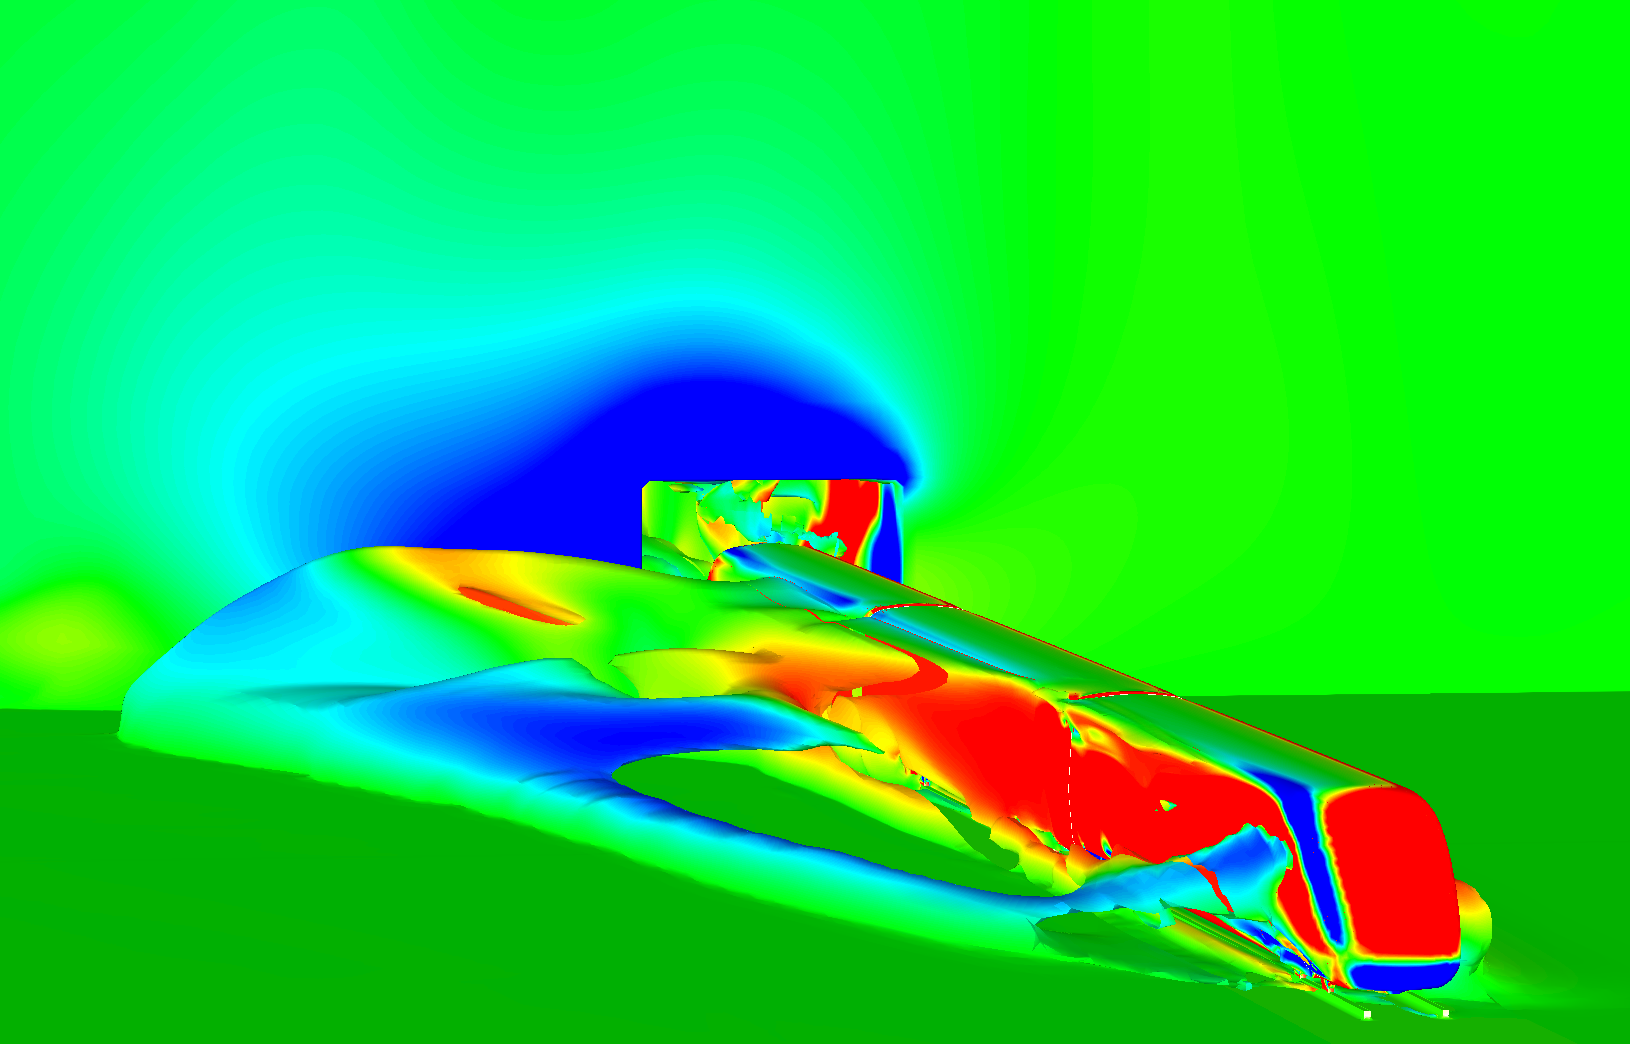
\includegraphics[width=\textwidth,height=0.4\paperheight,keepaspectratio]{figures/ExampleCover}}
\covercaption{Some explanation}

\firstabstract{\lipsum}
%\secondabstract{swedish}{\lipsum} % Optional
\keywords{Some stuff, More stuff, Stuff}

\preface{\lipsum} % You can use \input to put preface and acknowledgements in another document
\acknowledgements{\lipsum}
\dedication{\textit{to my dear mother.}}
\paperwork{\lipsum}

% You can add extra contents such as abbreviations and nomenclature using.
% Use \presectiontitle to render add titles to new sections.
\extrafrontmatter{\presectiontitle{Nomenclature} \lipsum} % Optional

\addbibresource{exampleBib.bib}


\begin{document}
%\makethesisdefence \end{document} % Should be printed at a5paper size
\maketitle


\part{Extended Summary}
\subfile{kappa}
\printbibliography

\part{Appended Papers A--B}
\fancyhf{} % to remove further pagenumbering
% paper A
\paper{\citefield{paper:A}{title}}{\fullcite{paper:A}}

\includepdf[pages=-,width=\paperwidth]{appendedPapers/paperA.pdf}

% paper B
\paper{\citefield{paper:B}{title}}{\fullcite{paper:B}}

\includepdf[pages=-,width=\paperwidth]{appendedPapers/paperB.pdf}

% bibliography of concrete structure/steel and timber.
\cleardoublepage

\includepdf[pages=-,width=\paperwidth]{appendedPapers/placeholder.pdf}
\end{document}
